%
% ginv.tex -- Invertierung des Gram-Operators
%
% (c) 2019 Prof Dr Andreas Müller, Hochschule Rapperswil
%
\section{Invertierung des Gram-Operators\label{section:ginv}}
\rhead{Invertierung des Gram-Operators}
\index{Invertierung des Gram-Operators}
Die Bestimmung des dualen Frame setzt voraus, dass der Gram-Operator
$G$ invertiert werden kann.
Eine linksinverse Transformation zum Frameoperator $M$ ist dann durch
$S=G^{-1}T^t$ gegeben.

Da $G$ eine positiv definite symmetrische Matrix mit Spektrum im
Intervall $[A,B]$ ist, ist die Matrix in der Eigenbasis sehr einfach
zu invertieren.
Die Eigenvektoren zu finden ist jedoch eine noch deutlich aufwendigere
Aufgabe, als die Matrix $G$ zu invertieren.
Ausserdem gibt es kein Interesse, in der Eigenbasis zu arbeiten, alle
Operationen sollen in der durch das Frame vorgegebenen Basis durchgeführt
werden.

Eine Linksinverse von $T$ zu finden ist gleichbedeutend damit,
die dualen Framevektoren $b_i' = Sb_i = G^{-1}Tb_i$ zu bestimmen.
Ziel dieses Abschnitts ist daher, einen spezialisierten numerischen
Algorithmus zu finden, der jeden der Vektoren $b_i'$ finden kann.

In der Eigenbasis von $G$ läuft die Invertierung von $G$ auf
das Invertieren der Eigenwerte hinaus.
Wir suchen daher in \ref{subsection:reziprok} erst einen iterativen
Algorithmus, der $1/\lambda$ berechnen kann für $\lambda\in[A,B]$.
In \ref{subsection:ginv} verallgemeinern wir diesen Algorithmus
anschliessend auf die Bestimmung von $G^{-1}$ bzw.~$b_i'$.

\subsection{Iterative Berechnung eines reziproken Wertes
\label{subsection:reziprok}}
Zu einer beliebigen Zahl $y$ mit $A < y < B$ muss der reziproke Wert $1/y$
bestimmt werden.
Wir suchen nach einem iterativen Verfahren der Form $x_{n+1}=f(x_n)$,
welches für einen beliebigen Startwert $x_0$ gegen $y^{-1}$ konvergiert
aber die Division nicht verwendet (da die Bestimmung der inversen
Matrix ja vermieden werden soll).
Der Wert $y^{-1}$ muss also der einzige Fixpunkt der Funktion $f(x)$ sein:
$f(y^{-1}=y^{-1}$.

Die Funktion $f(x) = x + g(x)$ hat als einzigen Fixpunkt die Stelle $x=y^{-1}$
genau dann, wenn $g(x)$ als einzige Nullstelle die Stelle $x=y^{-1}$ hat.
Ausserdem muss die Funktion $g(x)$ berechenbar sein ausschliesslich mit
Addition und Multiplikation von Konstanten und der Variablen $x$, Division
darf nicht verwendet werden.
Die einfachste Funktion dieser Art ist eine lineare Funktion, zum 
Beispiel $g(x) = 1- xy$.

\begin{figure}
\centering
\begin{tabular}{cc}
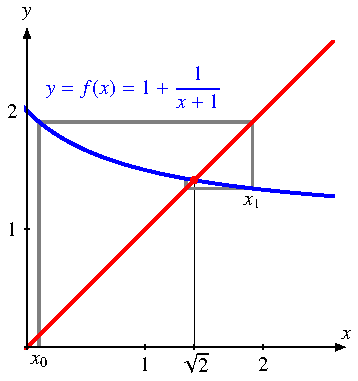
\includegraphics{chapters/1a-frames/images/ibkonv.pdf}&
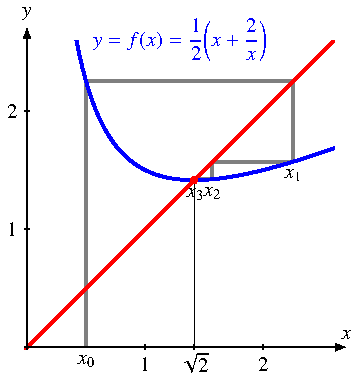
\includegraphics{chapters/1a-frames/images/itkonv.pdf}\\
(a)&(b)
\end{tabular}
\caption{Konvergenzeigenschaften eines Iterationsverfahrens der Form
$x_{n+1}=f(x_n)$.
Die Konstruktion des grauen Pfades ist im Text auf
Seite~\pageref{frame:grauerpfad} erklärt.
In beiden Fällen ist $\bar{x}=\sqrt{2}$ ein Fixpunkt der Funktion $f$.
Falls $|f'(\bar{x})| < 1$ konvergiert die Iterationsfolge linear, wie in (a)
erkennbar.
Für $f'(\bar{x})=0$ ist die Konvergenz besonders schnell (quadratische
Konvergenz), wie man in (b) sehen kann.
\label{frame:iterationsvergleich}}
\end{figure}

\begin{figure}
\centering
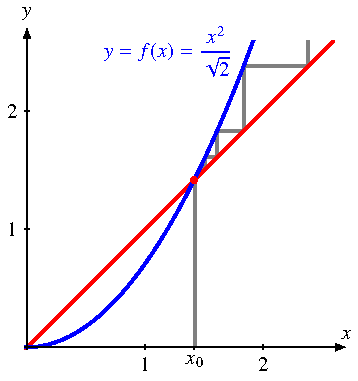
\includegraphics{chapters/1a-frames/images/div.pdf}
\caption{Konvergenzeigenschaften eines Iterationsverfahrens der Form
$x_{n+1}=f(x_n)$.
Für $|f'(\bar{x})|>1$ divergiert die Iterationsfolge (c).
\label{frame:divergenz}}
\end{figure}

Damit das Iterationsverfahren konvergiert, sind aber noch weitere
Bedingungen zu erfüllen (Abbildungen~\ref{frame:iterationsvergleich}
und \ref{frame:divergenz}).
Das Konvergenzverhalten kann wie folgt visualisiert werden.
Die Auswertung der Funktion $\color{blue}f(x_n)$ zeigen wir durch
eine Strecken von $(x_n,x_n)$ nach $\color{blue}(x_n,f(x_n))$ auf
dem blauen Graphen der Funktion $f$.
Die nächste Iteration startet mit $x_{n+1} = f(x_n)$, wir illustrieren
dies durch eine Strecke zum Punkt $\color{red}(f(x_n),f(x_n))$ auf der
Winkelhalbierenden des ersten Quadranten.
Auf diese Weise entsteht der graue Pfad in den Abbildungen.
\label{frame:grauerpfad}
Er führt jeweils vom blauen Graphen horizontal zur Winkelhalbierenden
und von dort vertikal wieder zum blauen Graphen.

Aus den Abbildungen kann man die folgende Bedingung für die Konvergenz
ablesen, die sich auch streng beweisen lässt.
Die Folge $x_{n+1} = f(x_n)$ konvergiert nur, wenn die Steigung
der Funktion $f(x)$ in der Nähe des Fixpunktes Betrag $<1$ hat, 
also $|f'(x)|<1$.
Für die eben konstruierte Funktion trifft dies im Allgemeinen nicht zu,
es ist nämlich
\[
f'(x) = 1 + g'(x) = 1 - y
\]
Für $y>2$ wird nämlich $|f'(x)|'=|1-y| = y-1 >1$, so dass keine Konvergenz
mehr möglich ist.
Allerdings ist Konvergenz auch nicht für alle Werte von $y$ nötig, sondern
nur für Werte zwischen $A$ und $B$.
Das kann man mit Hilfe eines Skalierungsfaktors $c$ in der Iteration
\[
f(x) = x + c(1-yx)
\]
erreichen.
Die Ableitung wird damit
\[
f'(x) = 1-cy.
\]
$c$  muss also so gewählt werden, dass $|f'(x)|<1$ gilt für alle $y$
zwischen $A$ und $B$.
Dies bedeutet, dass
\begin{align*}
-1 &< 1-cy < 1 \\
-2 &< -cy < 0 \\
2 &> cy > 0 \\
\frac1c &> \frac{y}2 \\
\end{align*}
Diese Ungleichung muss für alle möglichen Werte für $y$ erfüllt sein,
also sowohl für $y=A$ also auch für $y=B$.
Man kann dies zum Beispiel dadurch erreichen, dass man
\[
\frac1c = \frac{A}2 + \frac{B}2
\qquad\Rightarrow\qquad
c = \frac{2}{A+B}
\]
setzt.

Damit haben wir jetzt ein Iterationsverfahren zur Berechnung des 
reziproken Wertes, welches wir im folgenden Satz zusammenfassen.

\begin{satz}
\label{satz:reziprok}
Ist $y$ eine reelle Zahl zwischen $A$ und $B$, $A\le y\le B$ dann
konvergiert die Folge
\[
x_{n+1} = x_n + \frac{2}{A+B}(1-yx_n), \quad x_0 = 0
\]
gegen den reziproken Wert $y^{-1}$ von $y$.
Die Differenz zwischen aufeinanderfolgenden Approximationen nimmt
in jedem Schritt um mindestens den Faktor $(B-A)/(B+A)<1$ ab.
\end{satz}

Die Fehler verhalten sich also wie eine geometrische Folge.
\index{geometrische Folge}%
Man nennt diese Art von Konvergenz, bei der der Fehler in jedem
Schritt um den gleichen Faktor kleiner wird auch {\em lineare Konvergenz},
\index{lineare Konvergenz}%
weil die Anzahl der korrekten Stellen in jedem Schritt um gleichen
Wert zunimmt.

\begin{proof}[Beweis]
Wir müssen uns nur noch mit der Aussage über die Konvergenz befassen.
Dazu berechnen wir die Differenz zweier aufeinanderfolgender
Approximationen 
\begin{equation}
\left.
\begin{aligned}
x_{n+1} &= x_n + \frac{2}{A+B}(1-yx_n) \\
x_n &= x_{n-1} + \frac{2}{A+B}(1-yx_{n-1}) 
\end{aligned}
\right\}
\quad\Rightarrow\quad
x_{n+1}-x_n
=
x_n - x_{n-1} -\frac{2y}{A+B}(x_n-x_{n-1})
=
\underbrace{
\biggl(1-\frac{2y}{A+B}\biggr)
}_{\displaystyle=\vartheta}
(x_n - x_{n-1}).
\end{equation}
Die Differenz wird also tatsächlich um den Faktor $\vartheta$ ab.
Wir schätzen diesen Faktor ab
\[
\vartheta
=
1-\frac{2y}{A+B} = \frac{A+B-2y}{A+B}
\qquad
\Rightarrow
\qquad
|\vartheta|
<
\biggl|\frac{A+B-2B}{A+B}\biggr|
=
\biggl|\frac{A-B}{A+B}\biggr|
=
\frac{B-A}{B+A}.
\]
Da $A>0$ folgt auch $\vartheta<1$.
\end{proof}

Aus der Abschätzung von $|x_{n+1}-x_n|$ kann auch der Fehler
abgeschätzt werden.
Es gilt nämlich
\[
\frac1y
-
x_n
=
\frac1y - x_{n+1} + (x_{n+1} - x_n)
=
\frac1y - x_{n+1} + (x_{n+1} - x_n)
=
\sum_{k=n}^\infty(x_{k+1}-x_k).
\]
Wegen
\[
|x_{k+1} - x_k|
\le
\vartheta | x_{k}-x_{k-1}|
\le
\vartheta^2 | x_{k-1}-x_{k-2}|
\le \dots
\le
\vartheta^{k-n} |x_{n+1}-x_{n}|
\]
wird der Fehler der Approximation
\begin{align*}
\biggl|
\frac1y
-
x_n
\biggr|
=
\biggl|
\sum_{k=n}^\infty(x_{k+1}-x_k)
\biggr|
&\le
\sum_{k=n}^\infty|x_{k+1}-x_k|
\\
&\le
\sum_{k=n}^\infty \vartheta^{k-n} \cdot |x_{n+1}-x_n|
\\
&=
\sum_{k=0}^\infty \vartheta^k \cdot |x_{n+1}-x_n|
\\
&=
\frac1{1-\vartheta}\cdot |x_{n+1}-x_n|
\le
\frac{\vartheta^n}{1-\vartheta} |x_1-x_0|
\end{align*}
mit Hilfe der Summenformel für eine geometrische Reihe.
\index{Summenformel für geometrische Reihe}%
\index{geometrische Reihe!Summenformel}%
Daraus kann man auch ablesen, dass der Fehler wie $\vartheta^n$ gegen $0$
geht.

Die eben erreichte Schlussfolgerung lässt sich allgemeiner für eine
beliebige Vektorfolge in $\mathbb R^s$ formulieren.
Wir stellen dies im folgenden Lemma bereit, da uns die Aussage
im nächsten Abschnitt bei der Berechnung der Inversen von $G$ 
von Nutzen sein wird.

\begin{lemma}
\label{lemma:konvergenz}
Ist $x_n\in\mathbb R^s$ eine Folge mit der Eigenschaft, dass 
\[
|x_{n+1}-x_n| \le \vartheta\cdot|x_n-x_{n-1}|
\qquad
\forall n > 0,
\]
mit $0 < \vartheta  < 1$, dann konvergiert die Folge $x_n$ geometrisch
gegen einen Vektor $x\in\mathbb R^s$.
\end{lemma}

\begin{proof}[Beweis]
Um zu zeigen, dass die Folge konvergiert, muss man sich zunächst überzeugen,
dass die Folge $x_n$ eine Cauchy-Folge ist.
Dazu berechnen wir
\begin{align*}
|x_n-x_m|
&=
|x_n - x_{n-1}
     + x_{n-1} - x_{n-2}
               + \dots + x_{m+1} - x_m|
\\
&\le
|x_n-x_{n-1}|
+
|x_{n-1}-x_{n-2}|
+\dots+
|x_{m+1}-x_{m}|
\\
&\le
(
\vartheta^{n-m-1}
+
\vartheta^{n-m-2}
+
\dots
+
1
)
|x_{m+1}-x_{m}|
\\
&=
\frac{1-\vartheta^{n-m}}{1-\vartheta}
\cdot
|x_{m+1}-x_{m}|
\\
&\le 
\frac{1-\vartheta^{n-m}}{1-\vartheta}
\cdot
\vartheta^{m}
|x_{1}-x_{0}|
\le
\frac{\vartheta^m}{1-\vartheta}
|x_{1}-x_{0}|.
\end{align*}
Für eine Cauchy-Folge muss sichergestellt werden, dass die Differenz
$|x_n-x_m| <\varepsilon$ wird für genügend grosse Werte von $m$ und $n$.
Man muss also erreichen, dass
\begin{align*}
&&
\frac{\vartheta^m}{1-\vartheta} |x_1-x_0|
&\le \varepsilon
\\
&\Rightarrow&
\vartheta^m &\le \frac{|x_1-x_0|\varepsilon}{1-\vartheta}
\\
&\Rightarrow&
m\log \vartheta &\le \log \frac{|x_1-x_0|\varepsilon}{1-\vartheta}
\\
&\Rightarrow&
m&\ge \frac{1}{\log\vartheta}\cdot \log \frac{|x_1-x_0|\varepsilon}{1-\vartheta}
=
N(\varepsilon)
\end{align*}
Für jedes vorgegebene $\varepsilon>0$ kann man daher schliessen, dass
$|x_n-x_m|\le \varepsilon$ sobald $m,n>N(\varepsilon)$.
Damit ist gezeigt, dass $x_n$ eine Cauchy-Folge ist und damit in $\mathbb R^s$
einen Grenzwert hat, den wir mit $x$ bezeichnen.

Wir müssen jetzt noch nachweisen, dass $|x-x_n|$ geometrisch gegen $0$ geht.
Dazu berechnen wir
\begin{align*}
|x-x_n|
&=
|x-x_{n+1} + x_{n+1}-x_n|
\le |x-x_{n+1}| + |x_{n+1}-x_n|.
\intertext{Dies können wir $k-n$ mal iterieren, wobei $k>n$ sein muss,
und erhalten}
|x-x_n|
&\le |x - x_k| + \sum_{i=n}^{k-1} |x_{i+1} -x_{i}|
\\
&\le
|x-x_k| + \sum_{i=n}^{k-1} \vartheta^i |x_1-x_0|
=
|x-x_k| + |x_1-x_0|\vartheta^n \sum_{i=0}^{k-n-1}\vartheta^i.
\intertext{Die geometrische Reihe auf der rechten Seite kann man mit
der Summenformel für die geometrische Reihe vereinfachen und man erhält}
|x-x_n|
&=
|x-x_k|
+
|x_1-x_0|\vartheta^n \frac{1-\vartheta^{k-n}}{1-\vartheta}.
\end{align*}
Lässt man $k$ gegen $\infty$ gehen, verschwindet der erste Term auf
der rechten Seite, da ja $x_k\to x$.
Der verbleibende Ausdruck auf der rechten Seite ist
\begin{align*}
|x-x_n|
&\le
\vartheta^n
\frac{|x_1-x_0|}{1-\vartheta}.
\end{align*}
Der Bruch auf der rechten Seite hängt nicht von $n$ ab, wir bezeichen ihn
mit $a$.
Dann ist der Fehler der Approximation von $x$ durch $x_n$
\[
|x-x_n| \le a\vartheta^n,
\]
der Fehler geht also geometrisch gegen 0.
\end{proof}

\begin{figure}
\centering
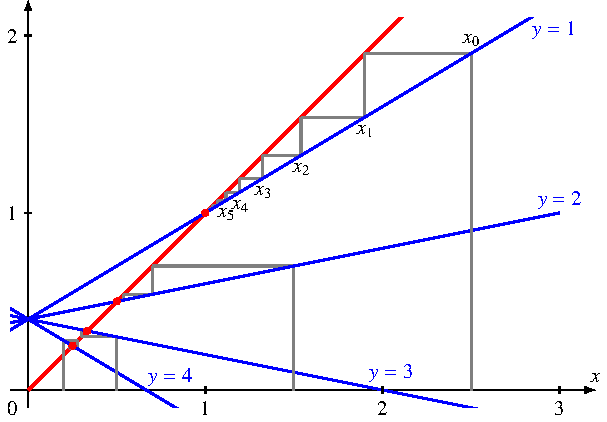
\includegraphics{chapters/1a-frames/images/iteration.pdf}
\caption{Iteration zur Bestimmung des Kehrwertes einer Zahl aus dem
Intervall $[1,5]$ mit der Iterationsformel
$x_{n+1} = f_y(x_n)=x_n + \frac13(1-yx_n)$.
Der Graph von $f_y(x)$ ist eine Gerade durch den Punkt $(0,\frac13)$.
Die Graphen für $f_1$, $f_2$, $f_3$ und $f_4$ sind blau eingezeichnet.
Die Iteration beginnend by einem Startwert $x_0$ führt auf einen 
grau dargestellten Pfad, der sich dem Fixpunkt $y^{-1}$ von $f_y(x)$
nähert.
\label{figure:reziprok}
}
\end{figure}

\begin{beispiel}
Wir verwenden das Verfahren, um den Wert von $1/3$ zu berechnen, also
für $y=3$.
Das Verfahren soll beliebige Werte zwischen $A=2$ und $B=5$ berechnen können.
Mit dem Startwert $x_0=0$ bekommen wir die Werte in
Tabelle~\ref{ginv:iteration:table}.
\begin{table}
\centering
\begin{tabular}{>{$}r<{$}|>{$}l<{$}}
n&x_n\\
\hline
 0&0.000000000000000\\
 1&0.285714285714286\\
 2&0.\underline{3}26530612244898\\
 3&0.\underline{33}2361516034985\\
 4&0.\underline{333}194502290712\\
 5&0.\underline{3333}13500327245\\
 6&0.\underline{33333}0500046749\\
 7&0.\underline{33333}2928578107\\
 8&0.\underline{333333}275511158\\
 9&0.\underline{3333333}25073023\\
10&0.\underline{33333333}2153289\\
11&0.\underline{333333333}164756\\
12&0.\underline{3333333333}09251\\
13&0.\underline{3333333333}29893\\
14&0.\underline{33333333333}2842\\
15&0.\underline{333333333333}263\\
16&0.\underline{3333333333333}23\\
17&0.\underline{33333333333333}2\\
18&0.\underline{333333333333333}\\
\end{tabular}
\caption{Iterative Berechnung von $\frac13$ mit Hilfe der Iterationsformel
von Satz~\ref{satz:reziprok}.
Korrekte Ziffern sind unterstrichen, in jedem Iterationsschritt nimmt
die Anzahl korrekter Ziffern um den gleichen Betrag zu, dies ist
lineare Konvergenz, der Fehler geht wie eine geometrische Folge
gegen $0$.
\label{ginv:iteration:table}
}
\end{table}
In jeder Iteration gewinnt man die gleiche Anzahl korrekter Stellen
(unterstrichen).
Aus dem Beweis von Satz~\ref{satz:reziprok} kann man ablesen,
dass die Konvergenzgeschwindigkeit
\[
\frac{A+B-2y}{A+B}
=
\frac{7-6}{7} = \frac17
\]
ist, man gewinnt also
$\log 7=0.84510$
Stellen in jeder Iteration, in Übereinstimmung mit den obigen numerischen
Resultaten.

Für jeden beliebigen Wert von $y$ im gegebenen Intervall ist die
Konvergenzgeschwindigkeit besser als
$\vartheta=3/7 = 0.42857142\dots$.
Die Anzahl Stellen, die man pro Iteration gewinnt ist daher 
$-\log\vartheta = 0.36798$.
Diese Konvergenzgeschwindigkeit erreicht man an den Enden des Intervalls.
Dazwischen kann man, wie oben gezeigt, deutlich schnellere Konvergenz haben.
\end{beispiel}

%
% Invertierung einer positiv definiten symmetrischen Matrix
%
\subsection{Invertierung einer positiv definiten symmetrischen Matrix $G$
\label{subsection:ginv}}
In diesem Abschnitt ist $G$ eine positiv definite symmetrische Matrix 
mit Eigenwerten im Intervall $[A,B]$.
In Satz~\ref{satz:reziprok} haben wir einen iterativen Algorithmus
gefunden, der jeden Eigenwert von $G$ invertieren kann.


\begin{satz}
\label{satz:ginv}
Ist $G$ eine positiv definite symmetrische Matrix mit Eigenwerten im
Intervall $[A,B]$ und $y\in\mathbb R^n$ dann konvergiert die Folge
\[
x_{n+1} = x_n + \frac{2}{A+B} (y - Gx_n),\qquad x_n = 0
\]
gegen 
$
x=\lim_{n\to\infty} x_n
$
mit $Gx=y$.
\end{satz}

\begin{proof}[Beweis]
Wie im Beweis von Satz~\ref{satz:reziprok} betrachten wir die
Iterationsfunktion
\[
f(x) = x + \frac{2}{A+B}(y-Gx),
\]
wobei $x\in\mathbb R^n$.
Wir müssen zeigen, dass diese Abbildung eine Kontraktion ist, dass
also der Abstand zwischen aufeinanderfolgenden Folgengliedern 
\begin{equation}
\left.
\begin{aligned}
x_{n+1} &= x_n + \frac{2}{A+B}(y-Gx_n)
\\
x_n &= x_{n-1} + \frac{2}{A+B}(y-Gx_{n-1})
\end{aligned}
\right\}
\quad
\Rightarrow
\quad
x_{n+1}- x_{n}
=
x_n-x_{n-1} \frac{2}{A+B}G(x_n-x_{n-1})
\label{inv:iteration:vector}
\end{equation}
in geometrischer Folge abnimmt.
Die rechte Seite von \eqref{inv:iteration:vector}
ist
\begin{equation}
x_n-x_{n-1} \frac{2}{A+B}G(x_n-x_{n-1})
=
\biggl(E-\frac{2}{A+B}G\biggr) (x_n-x_{n-1})
\label{inv:iteration:vector1}
\end{equation}
Wir müssen die rechte Seite abschätzen.
In einer Eigenbasis ist $G$ eine Diagonalmatrix mit Einträgen zwischen
$A$ und $B$.
Die grosse Klammer auf der rechten Seite von \eqref{inv:iteration:vector1}
ist in dieser Basis die Matrix
\[
E-\frac{2}{A+B}G
=
\begin{pmatrix}
1-\frac{2\lambda_1}{A+B} &            0             &\dots &        0         \\
          0              & 1-\frac{2\lambda_2}{A+B} &\dots &        0         \\
      \vdots             &          \vdots          &\ddots&     \vdots       \\
          0              &            0             &\dots & 1-\frac{2\lambda_n}{A+B}
\end{pmatrix}
\]
Die Einträge auf der Diagonalen sind
\begin{align}
1-
\frac{2 \lambda_i }{A+B}
&=
\frac{2}{A+B}
\biggl(
\frac{A+B}2 - \lambda_i
\biggr)
\label{inv:iteration:vector2}
\end{align}
Der Wert $(A+B)/2$ ist der Mittelpunkt des Intervalls $[A,B]$, die Eigenwerte
sind also höchstens die halbe Intervallänge $(B-A)/2$ vom Mittelpunkt
entfernt.
Die grosse Klammer auf der rechten Seite von~\eqref{inv:iteration:vector2}
ist daher betragsmässig höchstens $(B-A)/2$.
Nehmen wir den Betrag von~\eqref{inv:iteration:vector2}, erhalten wir
\[
\biggl|
1-
\frac{2 \lambda_i }{A+B}
\biggr|
\le 
\biggl|
\frac2{A+B}
\biggr|
\cdot \frac{B-A}2
=
\frac{B-A}{B+A}=\vartheta.
\]
Aus dem Beweis von Satz~\ref{satz:reziprok} ist bereits bekannt, dass
$0<\vartheta < 1$.

Aus \eqref{inv:iteration:vector} leiten wir jetzt ab, dass
\[
|x_{n+1} - x_n|
\le \vartheta |x_n-x_{n-1}|
\le \dots \le \vartheta^n |x_1-x_0|=\vartheta^n |x_1|.
\]
Die Unterschiede zwischen aufeinanderfolgenden Folgengliedern
nehmen also geometrisch ab.
Aus Lemma~\ref{lemma:konvergenz} folgt daher wie früher, dass
die Folge $(x_n)_{n\in\mathbb N}$ geometrisch gegen den Grenzwert
$x=\lim_{n\to\infty}$
konvergiert.

Wir müssen jetzt nur noch zeigen, dass $x$ tatsächlich das Bild von $y$
unter $G^{-1}$ ist.
Gehen wir in der Iterationsfolge zum Grenzwert über, folgt
\[
x_{n+1} = x_n + \frac{2}{A+B}(y-Gx_n)
\qquad\rightarrow\qquad
x = x + \frac{2}{A+B}(y-Gx).
\]
Die $x$ auf beiden Seiten des Gleichheitszeichens rechts
heben sich weg.
Den Faktor $2/(A+B)$ kann man wegkürzen, da er nie verschwindet.
Es bleibt
\[
0
=
y-Gx
\qquad
\Rightarrow
y=Gx,
\]
$x$ ist also der gesucht Urbildvektor.
\end{proof}

\begin{beispiel}
Wir verwenden die Iteration des Satzes \ref{satz:ginv} zur Berechnung
der Inversen der Matrix
\[
G=\begin{pmatrix}2&1&0\\1&2&1\\0&1&2\end{pmatrix}.
\]
Zunächst benötigen wir die Framekonstanten $A$ und $B$.
Diese müssen nicht exakt bekannt sein, es muss nur sichergestellt sein,
dass alle Eigenwerte $\lambda$ von $G$ im Intervall $[A,B]$ liegen.
Das charakteristische Polynom von $G$ ist
\[
\chi_{G}(\lambda)
=
\det(G-\lambda E)
=
\left|
\begin{matrix}
2-\lambda&1&0\\1&2-\lambda&1\\0&1&2-\lambda
\end{matrix}
\right|
=
(2-\lambda)^3-2(2-\lambda).
\]
Auf der rechten Seite lässt sich ein Faktor $(2-\lambda)$ ausklammern.
So erhält man
\begin{align*}
\chi_{G}(\lambda)
&=
(2-\lambda)\bigl((2-\lambda)^2-2\bigr)
=
(2-\lambda)
(\lambda^2 -4\lambda+2).
\end{align*}
Der quadratische Term auf der rechten Seite hat die Nullstellen
\[
\lambda_{\pm} = 2 \pm \sqrt{4-2} = 2 \pm\sqrt{2},
\]
damit kann man das charakteristische Polynom weiter faktorisieren
in
\[
\chi_{G}(\lambda)
=
(2-\lambda)
(\lambda -2-\sqrt{2})(\lambda -2+\sqrt{2}).
\]
Die Eigenwerte von $G$ sind daher
\[
2-\sqrt{2},\quad
2,\quad
2+\sqrt{2}.
\]
Die exakten Werte für $A$ und $B$ sind daher
\[
A=2-\sqrt{2}
\qquad\text{und}\qquad
B=2+\sqrt{2}.
\]
Der zugehörige Wert von $\vartheta$, der die Konvergenzgeschwindigkeit
definiert, ist $\vartheta = (A-B)/(A+B)=2\sqrt{2}/4=\sqrt{2}/2=0.707$.
Man leitet daraus ab, dass für jede Stelle Genauigkeit 6 Iterationsschritte
benötigt.
Für ein auf 5 Stellen exaktes Resultat muss man daher mit mindestens 30
Iterationsschritten rechnen.

Die Iterationsformel ist in beiden Fällen
\[
x_{n+1} = x_n + \frac12(y-Gx_n)
\]
mit Startwert $x_0=0$.
Für den ersten Standardbasisvektor $y=e_2$ findet man die Iterationsfolge
\begin{align*}
x_1 &=
\begin{pmatrix}
   0.0\\
   0.5\\
   0.0
\end{pmatrix},
&
x_2 &=
\begin{pmatrix}
  -0.25\\
 \phantom{-}  0.50\\
  -0.25
\end{pmatrix},
&
x_3 &=
\begin{pmatrix}
  -0.20\\
   \phantom{-}0.70\\
  -0.20
\end{pmatrix},
&
x_4 &=
\begin{pmatrix}
  -0.375\\
   \phantom{-}0.750\\
  -0.375
\end{pmatrix},
&
x_5 &=
\begin{pmatrix}
  -0.375\\
   \phantom{-}0.875\\
  -0.375
\end{pmatrix},
\\
x_6 &=
\begin{pmatrix}
  -0.4375\\
   \phantom{-}0.8750\\
  -0.4375
\end{pmatrix},
&
x_7 &=
\begin{pmatrix}
  -0.4375\\
   \phantom{-}0.9375\\
  -0.4375
\end{pmatrix},
&
x_8 &=
\begin{pmatrix}
  -0.46875\\
   \phantom{-}0.93750\\
  -0.46875
\end{pmatrix},
&
x_9 &=
\begin{pmatrix}
  -0.46875\\
   \phantom{-}0.96875\\
  -0.46875
\end{pmatrix},
&
x_{10} &=
\begin{pmatrix}
  -0.48438\\
   \phantom{-}0.96875\\
  -0.48438
\end{pmatrix},
\dots
\end{align*}
Die relative langsame Konvergenz kann gut verfolgt werden.
Der Grenzwert ist
\[
x_{\infty} = \lim_{n\to\infty}x_n = \begin{pmatrix}
-0.5\\\phantom{-}1.0\\-0.5
\end{pmatrix}.
\]
Führt man die Iteration für die anderen Standardbasisvektoren durch,
findet man als Grenzmatrix
\[
H=\frac14\begin{pmatrix}
 3&-2& 1\\
-2& 4&-2\\
 1&-2& 3
\end{pmatrix}
\]
und man kann leicht nachprüfen, dass $GH=E$.
\end{beispiel}

Im Beispiel wurde jeder Standardbasisvektor einzeln invertiert.
Dabei wurde immer die gleiche Operation
\[
x = x - \frac{2}{A+B}(y - Gx)
\]
angewendet.
Schreibt man alle Standardbasisvektoren in eine Matrix erhält man 
die Einheitsmatrix $E$. Aus den zugehörigen Vektoren $x_n$
wird die Matrix $H_n$, dann lässt sich die Operation auch als
Matrizenoperation
\[
H \to H - \frac{2}{A+B}(E - GH)
\]
schreiben.
Da jede einzeln Spalte mit der gleichen, durch $\vartheta = (B-A)/(B+A)$
definierten Geschwindigkeit konvergiert, kann der Satz auch als
Iterationsverfahren für die inverse Matrix formuliert werden.

\begin{satz}
Ist $G$ eine symmetrische Matrix derart, dass ihre Eigenwerte im
Intervall $[A,B]$ mit $0<A\le B$ enthalten sind, dann konvergiert
die Matrixfolge
\[
H_{n+1}
=
H_n
+
\frac{2}{A+B}
(
E-
GH_n
)
,
\qquad
H_0=0
\]
linear gegen den Matrix $H$ mit der Eigenschaft $GH=E$.
Der Fehler nimmt in jeder Iteration mindestens um den Faktor
$\vartheta=(B-A)/(A+B)$ ab.
\end{satz}








